\documentclass[11pt, twocolumn]{article}
\usepackage{graphicx}

\title{The exponential function}
\author{Mie Louise Lauridsen}
\date{March 3 2022}

\begin{document}

\maketitle

\section{Introduction}
The exponential function is a mathematical function. The function is denoted by $f(x)=\exp(x)$ of $e^x$. Its ubiquitous occurrence in pure and applied mathematics led mathematician Walter Rudin to opine that exponential function "\textit{the most importent function in mathematics}".(wiki) 

\section{Math}
The exponential function can be implemented by a "quick-and-dirty" method:
\begin{equation} \label{eq:exp}
\exp(x) = \sum_{k = 0}^{\infty} \frac{x^k}{k!} = 1 + x + \frac{x^2}{2} + \frac{x^3}{6} + \frac{x^4}{24} + \cdots
\end{equation}
Here the leading 10 orders has been included. In order to validate the function in equation (\ref{eq:exp}), has the exponential function been compared to table values. This can be seen on figure \ref{fig:exp}.

\begin{figure} [b]
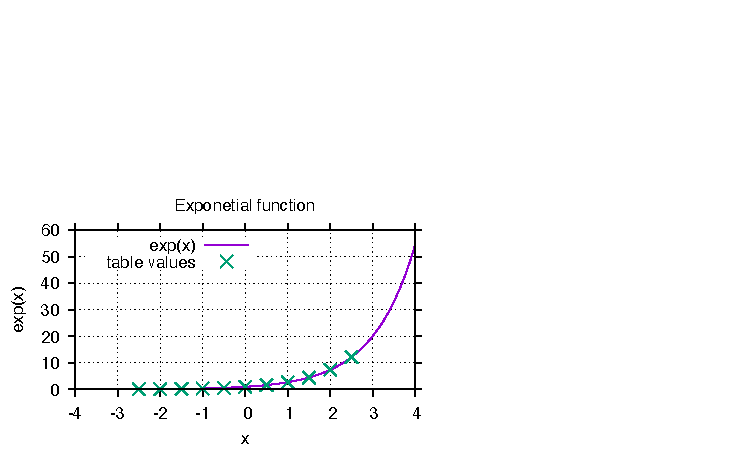
\includegraphics{exp_gnuplot.pdf}
\caption{Validation of the exponetial function.}
\label{fig:exp}
\end{figure}



\end{document}


